\section{Existing Work}
\label{Sec:RelatedWorks}

\begin{figure*}[h]
\centering
\subfloat[Naive Burst Buffer Aware Scheduler] {
        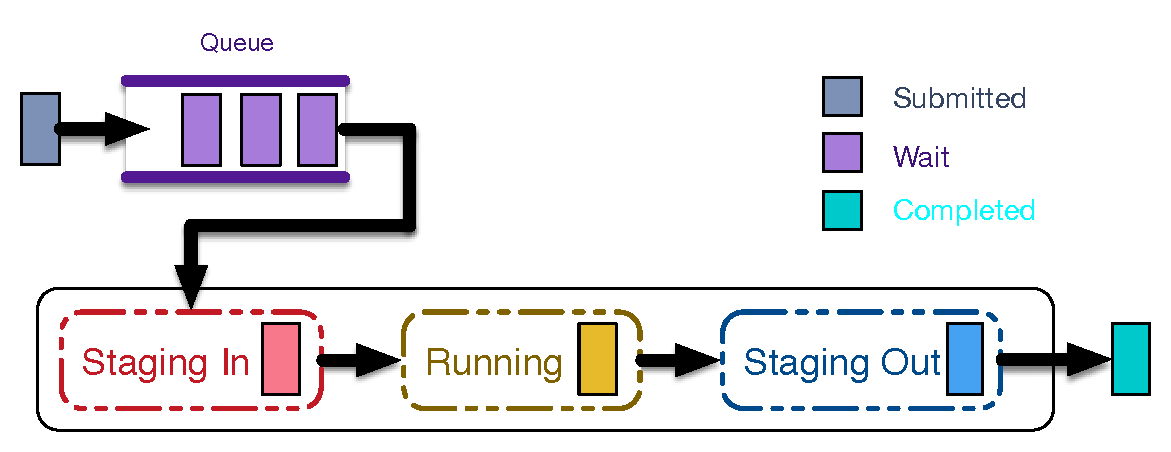
\includegraphics[width=3.1in]{SlurmQueue}
        \label{Fig:SlurmQueue}
}
\subfloat[Cerberus] {
        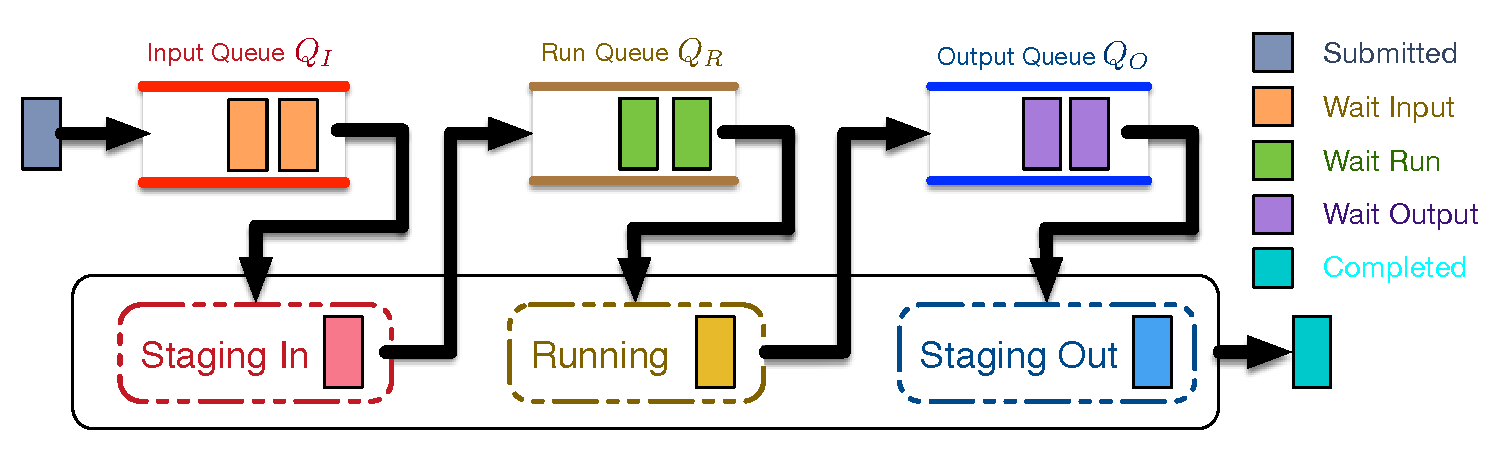
\includegraphics[width=3.7in]{CerberusQueues}
        \label{Fig:CerberusQueues}
}
\caption{}
\label{Fig:CompareSlurmCerbuers}
\end{figure*}

Given the critical role of burst buffer in future HPC systems,
users are encouraged to explicitly request this new resource for performance enhancement\cite{apex-workflow}.
Inspired by this requirement, it is necessary to holistically manage
the allocation of these precious I/O resources,
which naturally falls into the responsibilities of the batch scheduler.
Existing batch schedulers \cite{Moab, Cobalt, SlurmBBGuide, PBSonCRAY} have already claimed to
be aware of burst buffer, but in fact only deals with it in a naive way.

Figure~\ref{Fig:SlurmQueue} depicts the way existing burst-buffer-aware scheduler manages burst buffer.
For example, SLRUM developed a module that allocates burst buffer resources to the submitted user jobs.
The module extra considers if jobs' burst buffer requirements are meet when making scheduling decision.
With the pre-allocated burst buffer,
the I/O performance of user jobs indeed can be improved\cite{SlurmBBGuide}.
PBS supports burst buffer aware scheduling in similar way as SLURM:
jobs are only dispatched when both required burst buffer and computing resource are ready\cite{PBSonCRAY}.

However, there are three problems in such single-queueing scheduling framework.
First, even though job's lifetime is conceptionally be divide into 3 phases
(e.g. staging in, running and staging out), to the existing batch scheduler,
they are in fact just one running phase because scheduler cannot do anything once job is kicked off.
Secondly, a dispatched job will keep taking up its computing nodes and burst buffer nodes during its entire execution duration.
One may argue that there are cases that a job only need burst buffer to do I/O operations,
and there are cases that job can release computing nodes as soon as computation results is buffered
in burst buffer.
Finally, burst buffer and computing nodes are allocated altogether in the straightforward first-come, first-served manner, without doing any optimization.
In conclusion, the static burst-buffer-aware scheduling framework in Figure~\ref{Fig:SlurmQueue}
is far from fully exploiting the utilization of burst buffer.

This paper aims to bridge the two isolated fields of HPC architecture:
the novel burst buffer equipped HPC I/O subsystem and the
traditional batch job queueing subsystem.
The bridge builds upon a three-phase job model motivated by critical use cases of burst buffer,
i.e., application's bursty I/O pattern and data pre-fetch/cache.
This three-phase job model enables our scheduler to adopt the scheduling framework
illustrated in Figure~\ref{Fig:CerberusQueues}.
Comparing with the existing batch scheduler like SLRUM and PBS,

We target intelligently assigning burst buffer as a new system resource to the submitted user jobs.
In our scheduling model, users are encouraged to provide the burst buffer demand when submitting the jobs.
Based on the possible usage cases of burst buffer, the execution of user jobs is modeled into three phases.
The user jobs request different resources in each phase.
We propose a new batch scheduler with burst buffer awareness, Cerberus,
making scheduling decisions for jobs in each specific phase.
We also integrate Cerberus with different optimization algorithms for the
objectives of maximizing the resource utilization and the system throughput.

In the following sections, we demonstrate that when burst buffer is intelligently allocated
by our novel batch scheduler, the benefit is far beyond the higher hardware transfer bandwidth.
The job execution is expedited by having their bursty I/O requests absorbed by burst buffer.
The job waiting time is reduced via the contracted input/output stage in the scheduling pipeline.
To our best knowledge, this is the first attempt to holistically schedule jobs
running on the new burst-buffer-enabled HPC systems.


%I/O contention in HPC systems draws a lot of attention in the community,
%because it is one of the major culprits for parallel applications and performance variability.
%Hashimoto et al. evaluate the performance variability of each job
%when the jobs run concurrently on the same physical computing server.
%They identify that the network I/O sharing contributes the most to
%the performance degradation \cite{hashimoto:ICNC:2012}.
%Dorier et al. analyze the I/O interference between two applications.
%They make quantified study about the performance improvement obtained
%by interrupting or delaying one application in order to avoid I/O contention \cite{dorier:IPDPS:2014}.
%Yildiz et al. \cite{yildiz:IPDPS:2016} explore the variou root causes
%of I/O interference in HPC storage systems.
%They find that in many situations, interference is the result of the bad flow control in the I/O path,
%but is not caused by a single bottleneck in one of its components.

%The solutions to alleviate I/O contention between concurrently
%running jobs have been proposed in several recent works.
%Lofstead et al. propose to individually schedule each application's I/O requests without
%a global view from the system's perspective \cite{lofstead:sc:2010}.
%Their solutions require the support from the specific I/O management
%in the system level to achieve good results.
%Zhou et al. design a new I/O aware batch scheduler to address the I/O
%contention problem at the batch scheduling level \cite{zhou:Cluster:2015}.
%The new scheduler coordinates the  I/O requests without hurting the fairness across applications.
%Liu et al. propose to move many file handling procedures to the I/O nodes to
%ameliorate the I/O pressure from the massive number of compute nodes\cite{Liu:MSST:2012}.

%SLURM develops a new module for its batch scheduler that allocates burst buffer
%resources to the submitted user jobs. With the pre-allocated burst buffer,
%the I/O performance of user jobs is greatly improved \cite{SlurmBBGuide}.
%However, the policy they used for the resource allocation is in a first-come, first-serve manner without optimization.
%PBS supports burst buffer aware scheduling in similar way as SLURM, 
%jobs are only dispatched when required burst buffer resource are ready\cite{PBSonCRAY}. 
%Their static burst buffer aware scheduling strategies would lead to low resource utilization.

%Our work is different from the existing research in the following ways.
%We target intelligently assigning burst buffer as a new system resource to the submitted user jobs.
%In our scheduling model, users are encouraged to provide the burst buffer demand when submitting the jobs.
%Based on the possible usage cases of burst buffer, the execution of user jobs is modeled into three phases.
%The user jobs request different resources in each phase.
%We propose a new batch scheduler with burst buffer awareness, Cerberus,
%making scheduling decisions for jobs in each specific phase.
%We also integrate Cerberus with different optimization algorithms for the
%objectives of maximizing the resource utilization and the system throughput.


% \cite{SlurmBBGuide}


